\documentclass[prb,preprint]{revtex4-1} 


\usepackage{amsmath}  
\usepackage{amsfonts} 
\usepackage{graphicx} 
\usepackage{color}
\usepackage{ulem}
\begin{document}


\title{Recreating Young's Double Slit Experiment}


\author{Ed Lipchus}
\email{ejl13@hampshire.edu}
\affiliation{Department of Natural Science, Hampshire College, Amherst, MA 01002}


\author{Danika Luntz-Martin}
\email{dluntzma@smith.edu}
\affiliation{Department of Physics, Smith College, Northampton, MA 01063}


\date{\today}



\begin{abstract}


\end{abstract}

\maketitle 


\section{Introduction} 

The double slit experiment preformed by Thomas Young was seminal because it demonstrated the wave nature of light. 

\section{Methods}

We used the TeachSpin Two-Slit Interference, One Photon at a Time (TWS1-B) which is a apparatus designed to perform Young's double slit experiment. The apparatus has two light sources, a 670 nm diode laser and a light bulb with a removable green light filter. There are four slit holders spaced throughout the length of the apparatus, see Figure~\ref{apparatus}. The first slit, the source slit, is eliminates excess light from the light source and approximates a plane wave. Next is the double slit, our double slit had 0.1mm wide slits and center to center separation of 0.353mm. Following the double slit was a wide single slit attached to a micrometer, called the slit blocker. The slit blocker could be moved to block either or both slits of the double slit. Finally there was a detector slit which allowed us to measure the intensity of light (using the laser) or the number of photons (using the light bulb) over a small region of the x-axis. The micrometer attached to the detector slit allowed us to scan along the x-axis. When we worked with the laser as our light source we used the built in photodetector which gave an output voltage that was proportionate to the light intensity. When we used light bulb as our light source we used the built in photo-multiplier tube (PMT) attached to the TeachSpin Pulse Counter / Interval Timer (PCIT1) to count the number of photons.


\begin{figure}[h!]
\centering
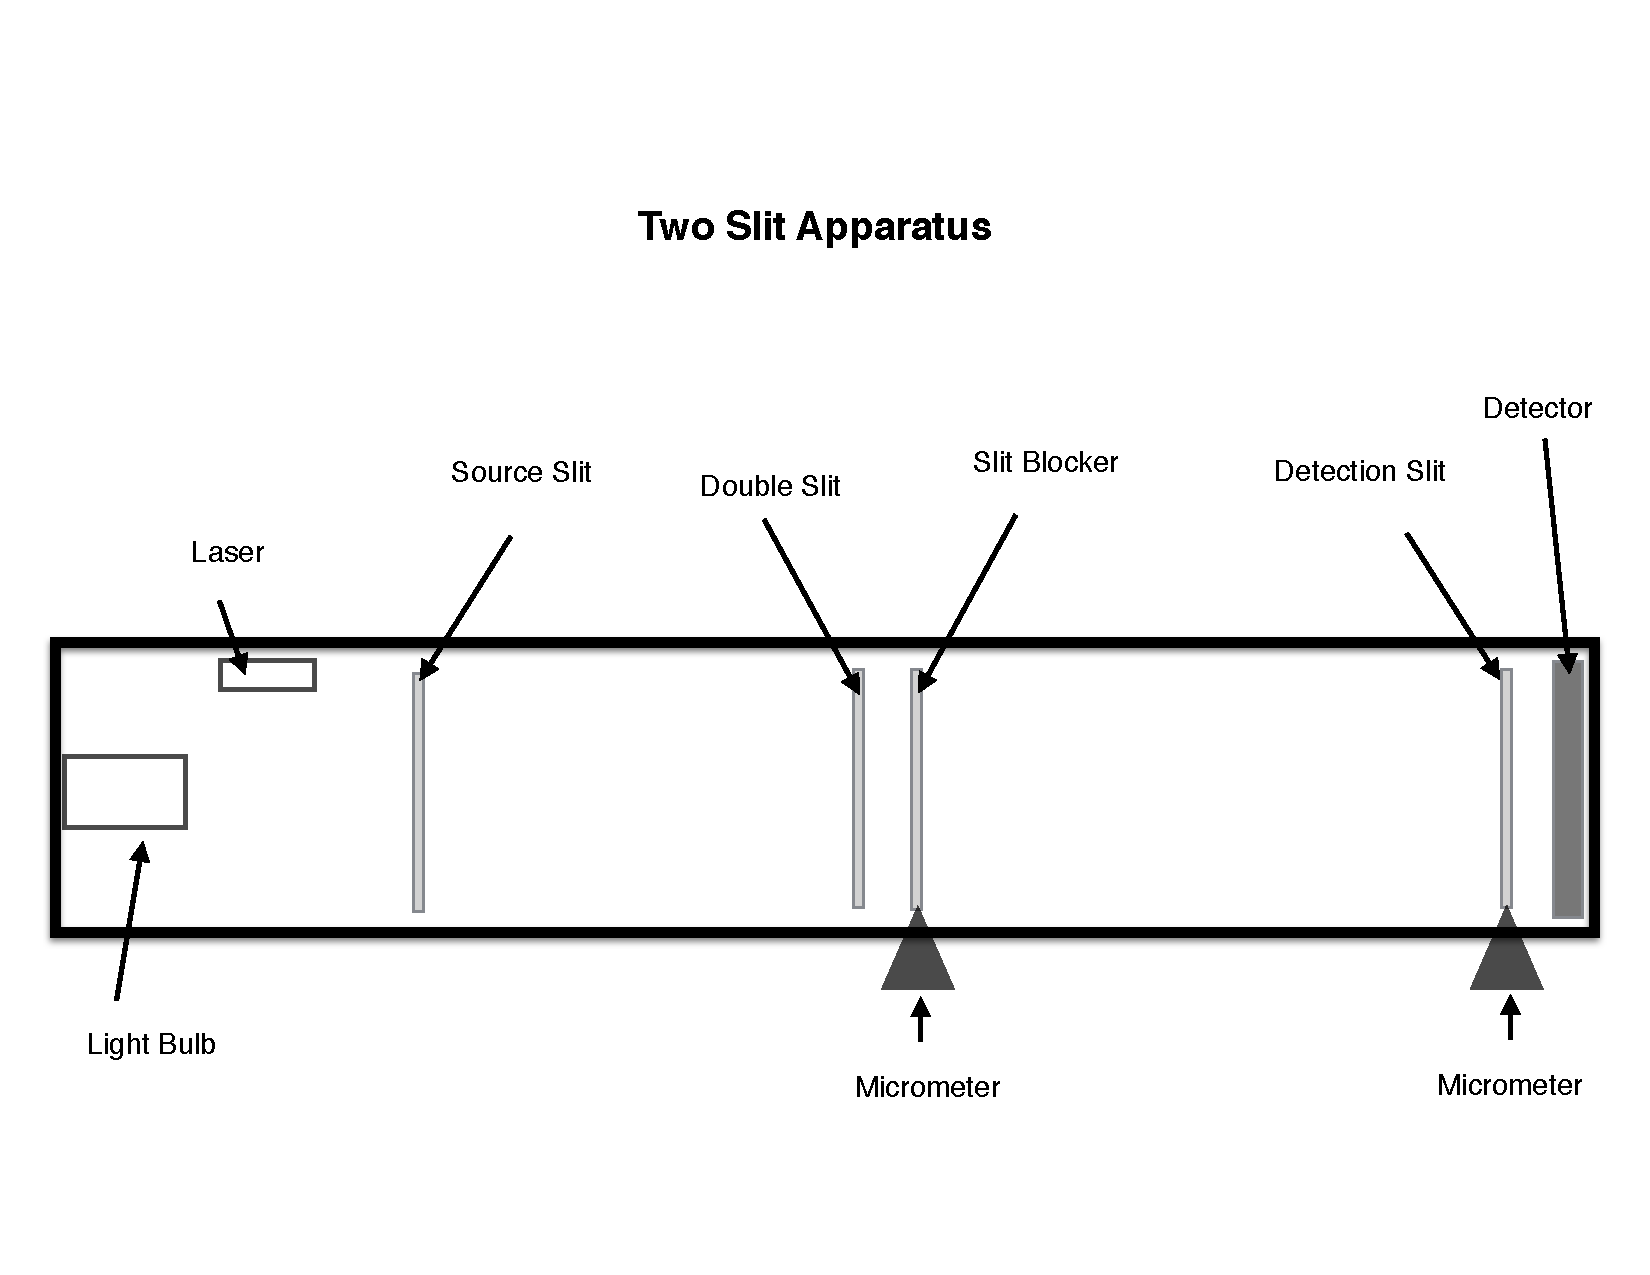
\includegraphics[width=6in]{apparatus.pdf}
\caption{The experimental set-up of the apparatus we used. The laser can slide into place in front of the light bulb. The source slit is a wide slit that blocks extraneous light from the light source. The slit blocker is another wide slit that can be moved, using the micrometer, to block one of the double slits, effectively turning it into a single slit. The detector slit allowed us to count the number of photon reaching the detector over a small region. The micrometer allowed us to scan across the detector and get a photon count at each x value.}
\label{apparatus}
\end{figure}


We began by aligning the slits within our apparatus. We started by using the laser roughly align the source slit and double slit and ensure that the double slit was not tilted. Then we made fine adjustments to the alignment using the light bulb. Throughout our experiments we used a midrange light bulb power setting of 5. We used a green filter on our light bulb to lower the intensity of the light and narrow the range of wavelengths to 541 - 551nm. 

Next we optimized the signal-to-noise ratio for our PMT. To do so we held the PMT voltage constant and varied the discriminator threshold. We found that dial value of the PMT voltage was not consistent with the measured value of the PMT voltage using a digital multimeter, so we used the multimeter reading to determine our voltage. For each value of the discriminator threshold we measured four values for our signal plus our noise and four values of just noise with no signal. We then averaged each set of four values and took the ratio to calculate the signal-to-noise. In our case the ratio we actually calculated was signal and noise to noise, this difference should scale our results but not change the overall outcome. The calculated signal-to-noise rations can be seen for various PMT voltages in Figure~\ref{signaltonoise}. The highest values for the PMT voltage, 900 V and 800 V, had a significantly lower signal to noise ratio. The lower values for the PMT voltage, 600 V and 650 V, required small values for the discriminator threshold and did not have as high a signal-to-noise ratio. The highest signal-to-noise ratio we obtained was for PMT voltage of 750 V and a discriminator threshold of 15.

\begin{figure}[h!]
\centering
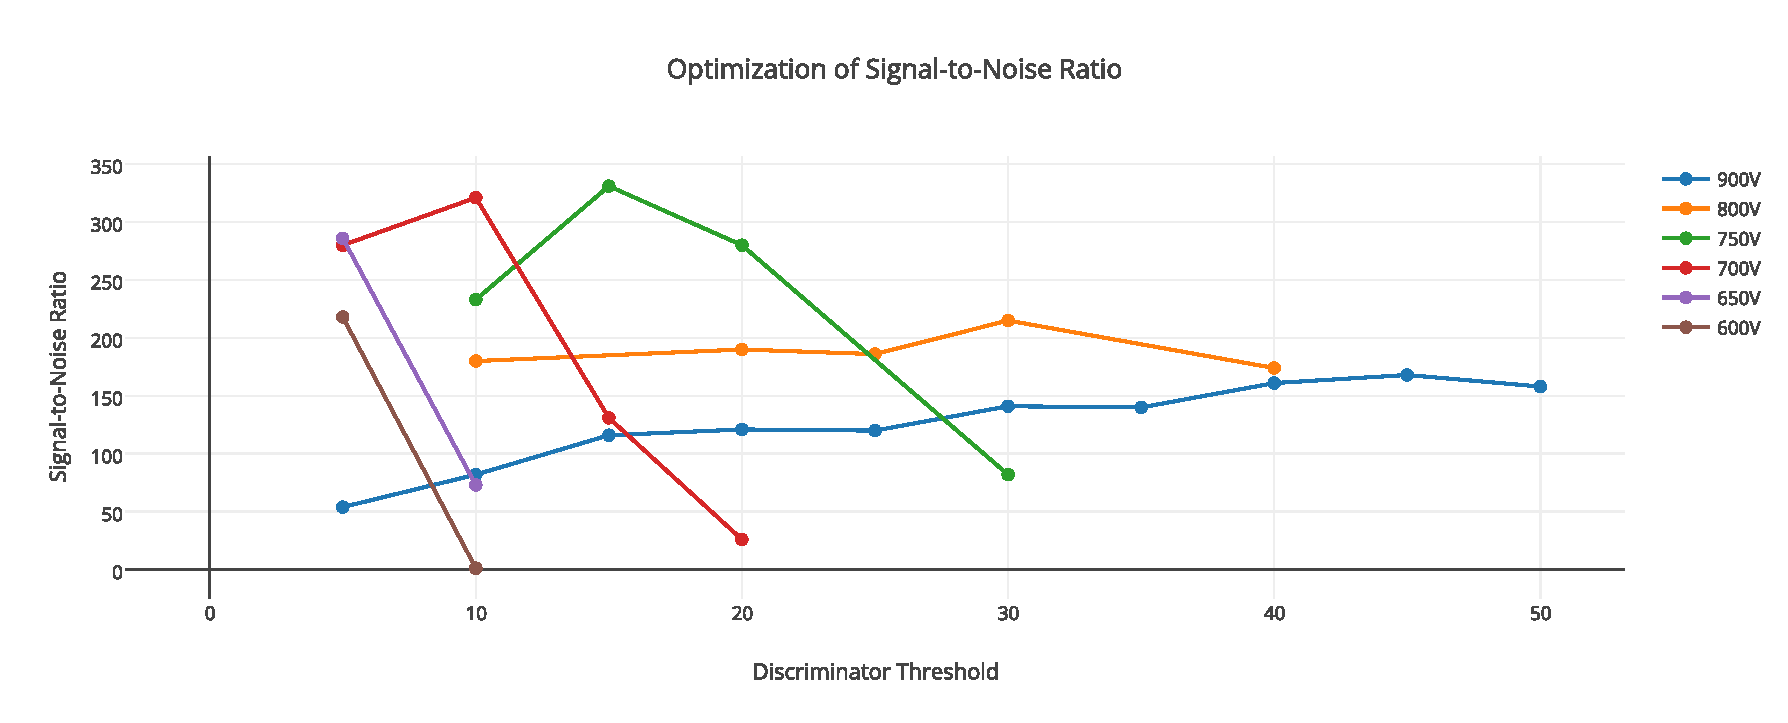
\includegraphics[width=6in]{signaltonoise.pdf}
\caption{The signal-to-noise ratios we obtained for a range of discriminator thresholds for various PMT voltages. For the high PMT voltages, 900 V (blue) and 800 V (orange) the signal-to-noise ratio was much lower. For lower PMT voltages, 650 V (purple) and 600 V (brown), the signal-to-noise ratio was again lower. The optimal signal-to-noise ratio was at a PMT voltage of 750 V (green) and a discriminator threshold value of 15.}
\label{signaltoniose}
\end{figure}

To collect data we used a Labview program called ``TeachSpin Counter V3'' that connected to the pulse counter. We then moved the detector slit along the x-axis in increments of 0.05 mm and recorded the number of counts given by the pulse counter. We were careful when collecting multiple sets of data to only scan along the x-axis in one direction and turn the micrometer father than necessary to minimize any backlash effects.

\section{Results}

We collected three sets of data using the double slit arrangement. Figure~\ref{doubleslit} shows a representative selection of the data we collected. The alignment of our slits was not exact because the minima at smaller x values do not reach zero. However, the vertical offset was not linear so it could not easily be subtracted off.

\begin{figure}[h!]
\centering
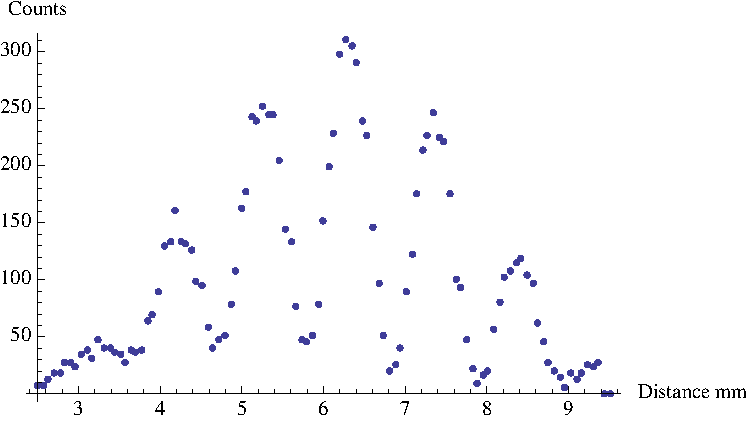
\includegraphics[width=6in]{doubleslit.pdf}
\caption{Data collected for the double slit arrangement. Our alignment was imperfect because the minima on the right side do not reach zero.}
\label{doubleslit}
\end{figure}

Using the slit blocker we were able to obtain single slit data from both the near and the far slits. We found further evidence of the misalignment of our slits. The intensity of the near slit, Figure~\ref{singlenear}, was one fourth of the intensity of the double slit arrangement which in is agreement with the theory. However the intensity of the far slit, Figure~\ref{singlefar}, was twice the intensity of the near slit and nearly twice the intensity predicted by theory. The discrepancy was mostly likely caused by our inability to exactly align the slits. It is also possible that the increase in intensity was caused by a reflection off the wall the apparatus that was was going around the silt instead of through them.

\begin{figure}[h!]
\centering
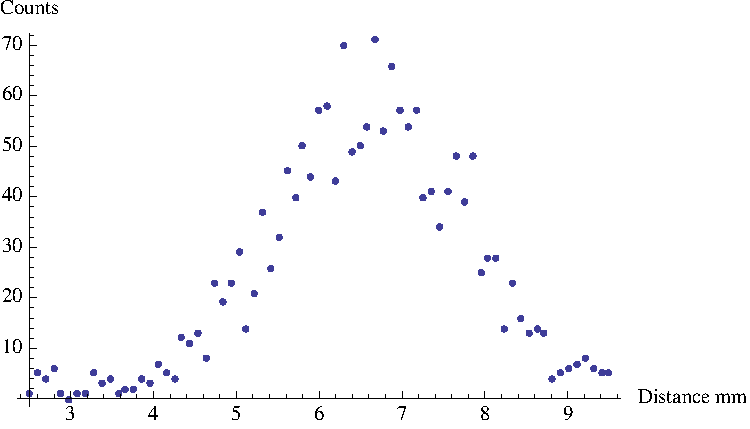
\includegraphics[width=6in]{singlenear.pdf}
\caption{Data collected for a single slit arrangement using the near slit. There appears to be a large uncertainty, note the wide band of data points. The intensity of the near single slit is approximately one fourth the intensity of the double slit.}
\label{singlenear}
\end{figure}

\begin{figure}[h!]
\centering
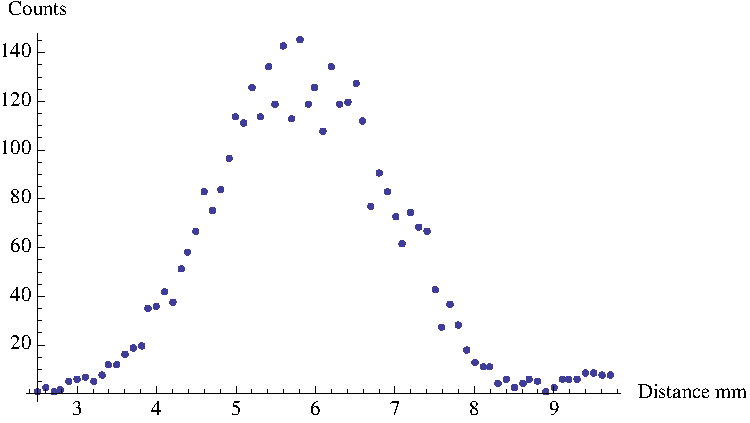
\includegraphics[width=6in]{singlefar.pdf}
\caption{Data collected for a single slit arrangement using the far slit. There is again a large uncertainty evident from the wide line of data points. The intensity of this slit is nearly twice the intensity of the near slit. This is mostly likely due to misalignment or reflected light from outside the slit.}
\label{singlefar}
\end{figure}


\section{Analysis}


\section{Discussion}


\section{Conclusion}

\begin{thebibliography}{1}

\bibitem{teachspin} Jonathan F. Reichert, \textit{TeachSpin Instruction Manuals: Two-Slit Interference, One Photon at a Time (TWS1 - B), Pulse Counter / Interval Timer (PCIT1)} Rev. 1.0, (2013)

\end{thebibliography}
\end{document}
